\documentclass[default]{beamer}
\setbeamertemplate{navigation symbols}{}

\usetheme{CambridgeUS}
\useoutertheme{infolines}
%\usecolortheme{crane}

\usepackage{cmap}	% Поддержка поиска русских слов в PDF (pdflatex)
\usepackage[T2A]{fontenc}       %поддержка кириллицы
\usepackage[utf8]{inputenc}	% Выбор языка и кодировки
\usepackage[english, russian]{babel}

\graphicspath{{../../images/3-control/}} 			% Пути к изображениям

\makeatletter
\setbeamertemplate{footline}
{
	\leavevmode%
	\hbox{%
		\begin{beamercolorbox}[wd=.333333\paperwidth,ht=2.25ex,dp=1ex,center]{author in head/foot}%
			\usebeamerfont{author in head/foot}\insertshortauthor~~\beamer@ifempty{\insertshortinstitute}{}{(\insertshortinstitute)}
		\end{beamercolorbox}%
		\begin{beamercolorbox}[wd=.333333\paperwidth,ht=2.25ex,dp=1ex,center]{title in head/foot}%
			\usebeamerfont{title in head/foot}\insertshorttitle
		\end{beamercolorbox}%
		\begin{beamercolorbox}[wd=.333333\paperwidth,ht=2.25ex,dp=1ex,right]{date in head/foot}%
			\usebeamerfont{date in head/foot}\insertshortdate{}\hspace*{2em}
			\insertframenumber{}\hspace*{2ex} 
		\end{beamercolorbox}}%
		\vskip0pt%
	}
\makeatother
	
\begin{document}
	
	\title[Многоуровневая система управления]{Многоуровневая система управления коалициями сложных технических объектов}
	\author[Макаров, Яковлев, Панов]{Дмитрий Макров, Константин Яковлев, Александр Панов}
	\institute[ИСА РАН]{Институт системного анализа РАН}
	\date{18 декабря 2014 г.} 

	\begin{frame}
		\titlepage
	\end{frame}

	\begin{frame}
		\frametitle{Общий вид архитектуры}
		\begin{figure}
			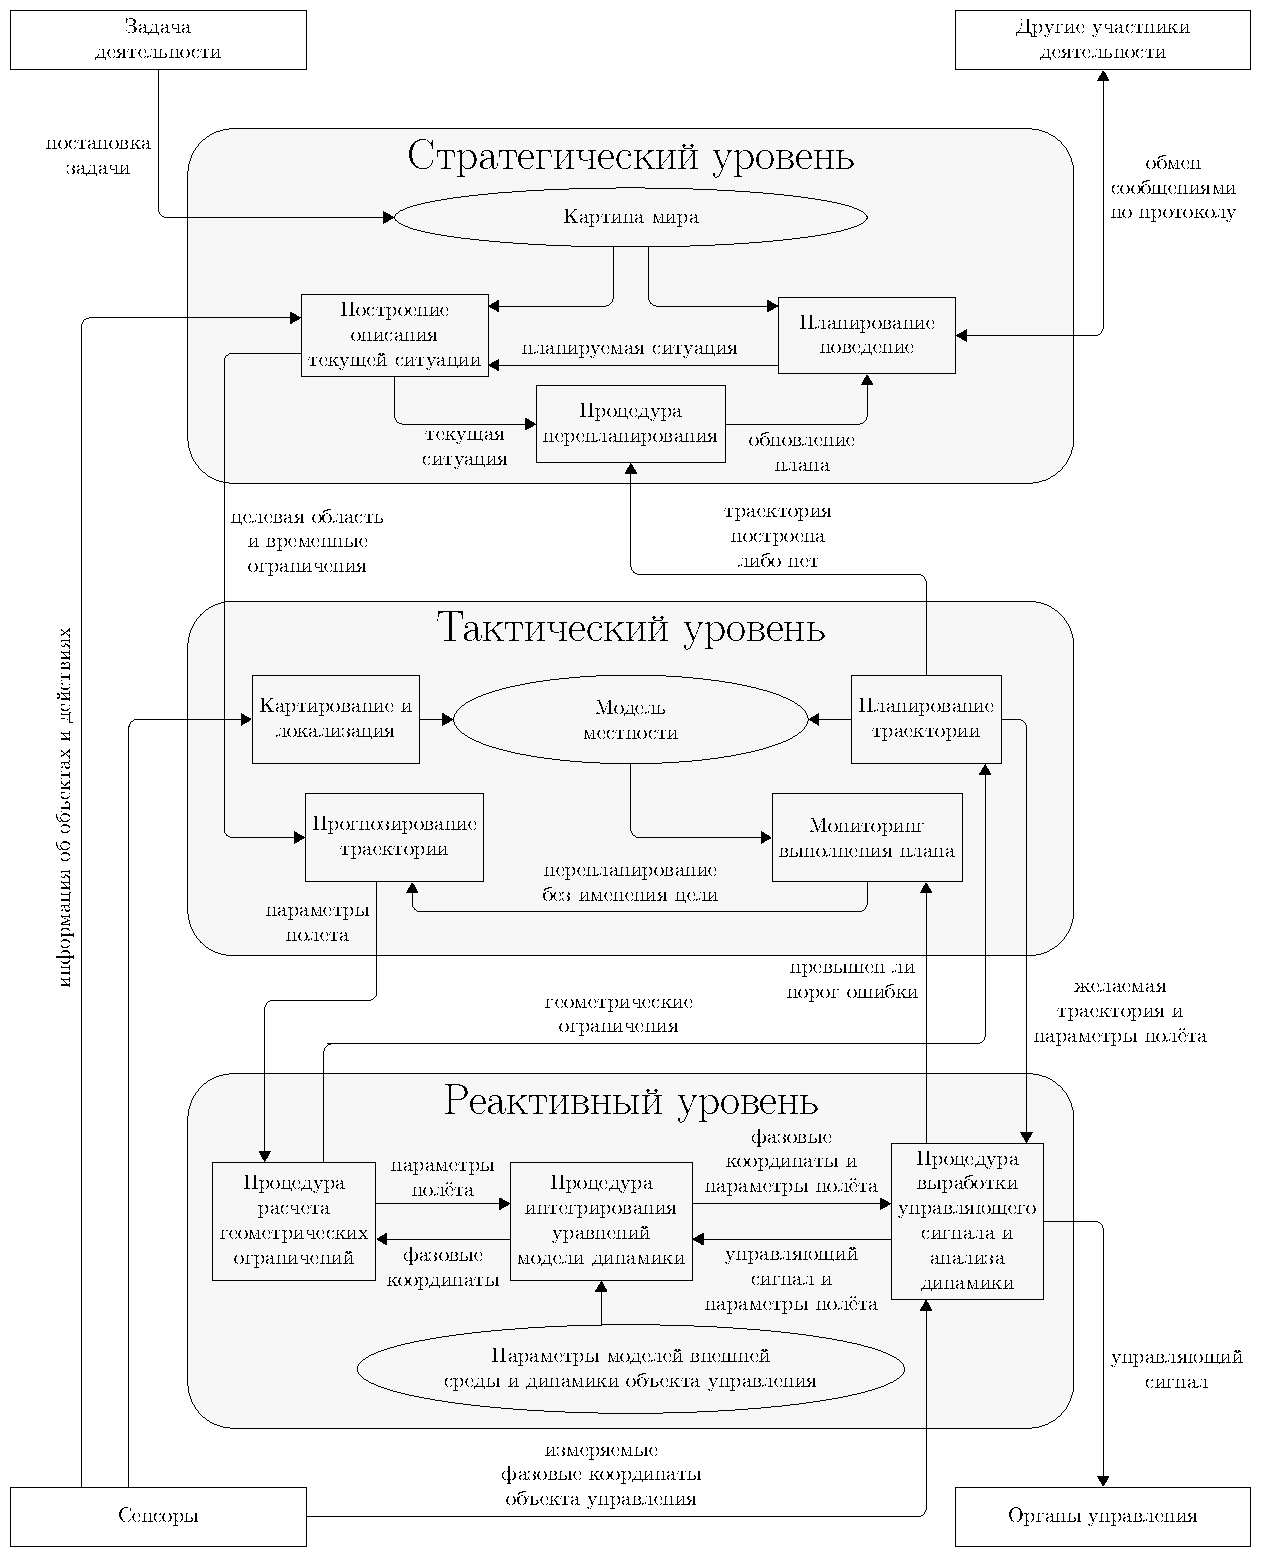
\includegraphics[width=0.5\textwidth]{../architecture}
		\end{figure}
	\end{frame}

	\section{Стратегический уровень}
		
	\begin{frame}
		\frametitle{Знаковая картина мира "--- новый способ представления знаний}
		\begin{columns}
			\begin{column}{0.5\textwidth}
				\begin{figure}
					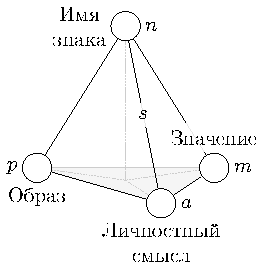
\includegraphics[width=0.8\textwidth]{../sign}
				\end{figure}
			\end{column}
			\begin{column}{0.5\textwidth}
				\begin{figure}
					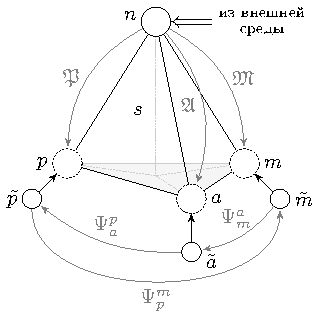
\includegraphics[width=0.8\textwidth]{../sign_naming}
				\end{figure}
			\end{column}
		\end{columns}
		\begin{columns}
			\begin{column}{0.5\textwidth}
				\begin{center}
					Структура знака.
				\end{center}
			\end{column}
			\begin{column}{0.5\textwidth}
				\begin{center}
					Процедура формирования знака.
				\end{center}
			\end{column}
		\end{columns}
	\end{frame}
	
	\begin{frame}
		\frametitle{Распознающий автомат "--- модель компонент знака}
			\begin{figure}
				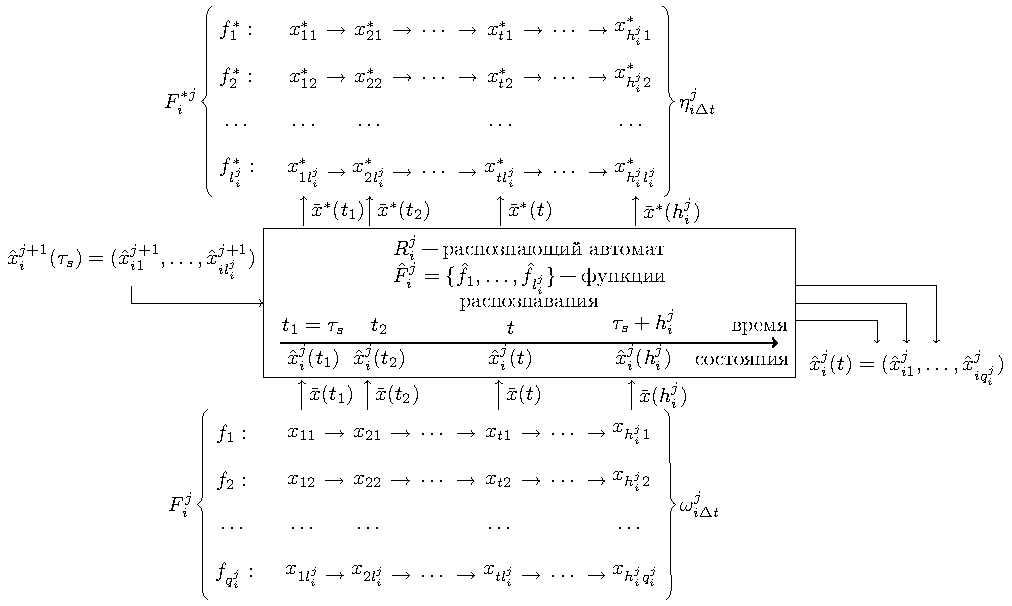
\includegraphics[width=0.7\textwidth]{../rb_io}
			\end{figure}

			$R$-автомат $R_i^j$ является бесконечным автоматом Миля с переменной структурой и конечной памятью и определяется следующим набором $R_i^j=<X_i^j\times \hat{X}_i^{j+1}, 2^{\mathcal Z_i^j}, X_i^{*j}\times \hat{X}_i^j,\varphi_i^j,\vec\eta_i^j>$.	
	\end{frame}

	\begin{frame}
		\frametitle{Процедуры самоорганизации и структуры на множестве знаков}
		\begin{columns}
			\begin{column}{0.5\textwidth}
				\begin{figure}
					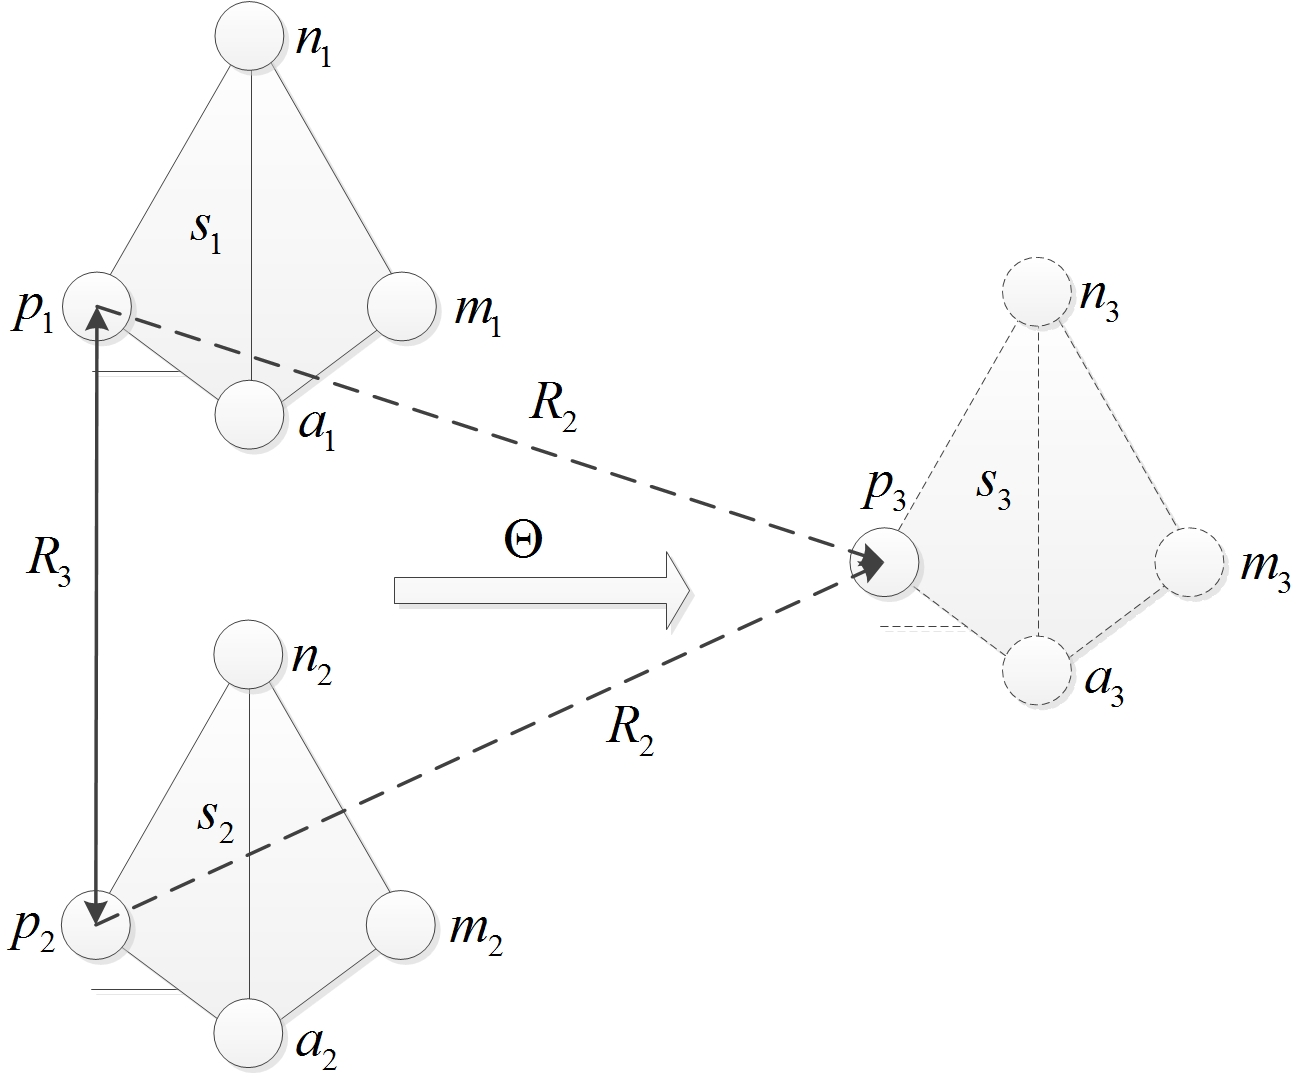
\includegraphics[width=0.8\textwidth]{../pattern_gen.jpg}
				\end{figure}
			\end{column}
			\begin{column}{0.5\textwidth}
				\begin{figure}
					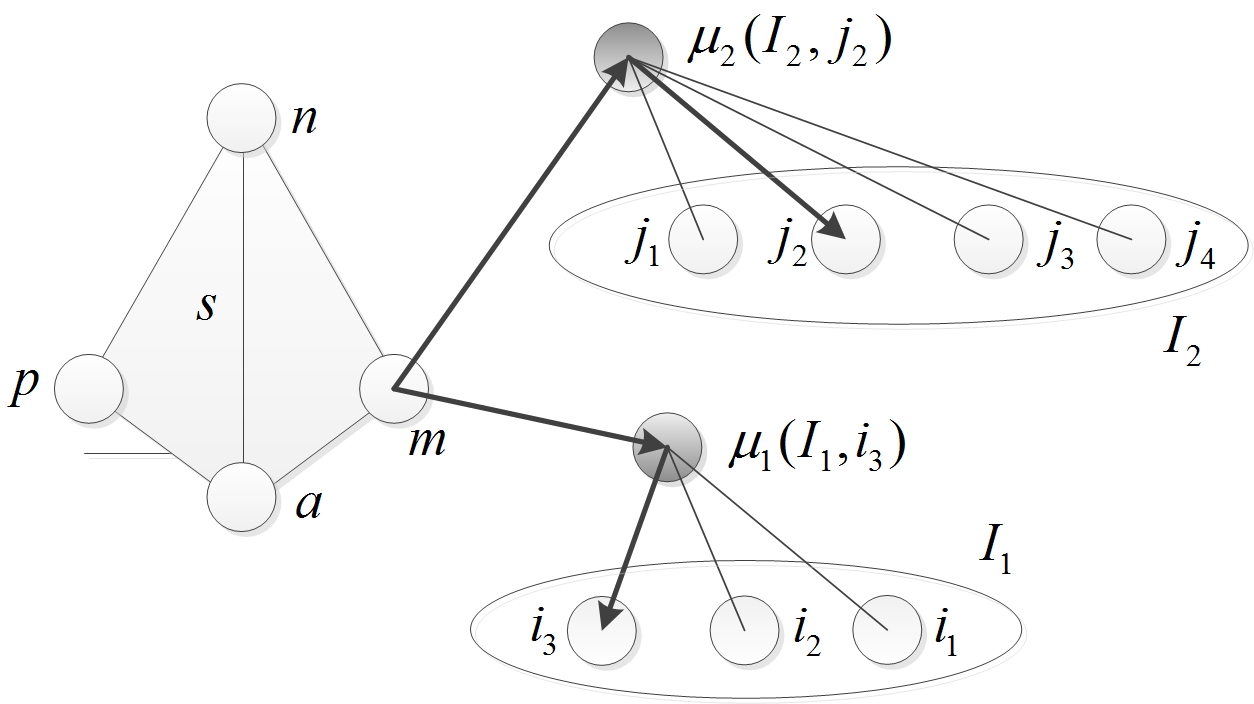
\includegraphics[width=0.9\textwidth]{../mean_scene.jpg}
				\end{figure}
			\end{column}
		\end{columns}
		\begin{columns}
			\begin{column}{0.5\textwidth}
				\begin{center}
					Обобщение по образам знаков с образованием нового знака.
				\end{center}
			\end{column}
			\begin{column}{0.5\textwidth}
				\begin{center}
					Сцена, образующаяся за счёт ролевой структуры действия, интерпретируемого экземпляром значения.
				\end{center}
			\end{column}
		\end{columns}
	\end{frame}
	
	\section{Тактический уровень}
		
	\begin{frame}
		\frametitle{Задача планирования как задача поиска пути на графе регулярной декомпозиции}
		\begin{columns}
			\begin{column}{0.6\textwidth}
				\begin{figure}
					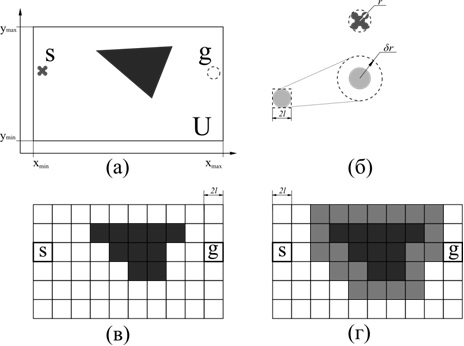
\includegraphics[width=\textwidth]{plan_1.jpg}
				\end{figure}
			\end{column}
			\begin{column}{0.4\textwidth}
				\begin{figure}
					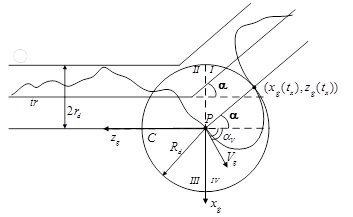
\includegraphics[width=\textwidth]{plan_2.jpg}
				\end{figure}
				\begin{figure}
					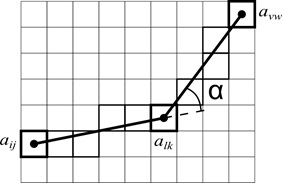
\includegraphics[width=0.8\textwidth]{plan_3.jpg}
				\end{figure}
			\end{column}
		\end{columns}
	\end{frame}
	
	\begin{frame}
		\frametitle{Алгоритм LIAN }
		\begin{columns}
			\begin{column}{0.5\textwidth}
				\begin{figure}
					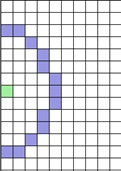
\includegraphics[width=0.3\textwidth]{lian_1.jpg}
				\end{figure}
			\end{column}
			\begin{column}{0.5\textwidth}
				\begin{figure}
					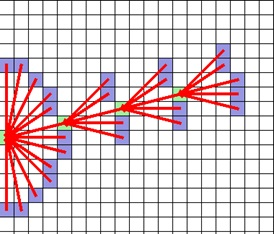
\includegraphics[width=0.5\textwidth]{lian_2.jpg}
				\end{figure}
			\end{column}
		\end{columns}
		\begin{figure}
			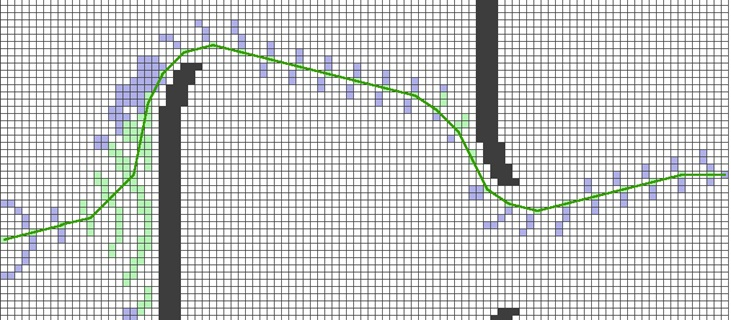
\includegraphics[width=0.8\textwidth]{lian_3.jpg}
		\end{figure}
	\end{frame}
	
	\begin{frame}
		\frametitle{Результаты экспериментов планирования траекторий}
		\begin{figure}
			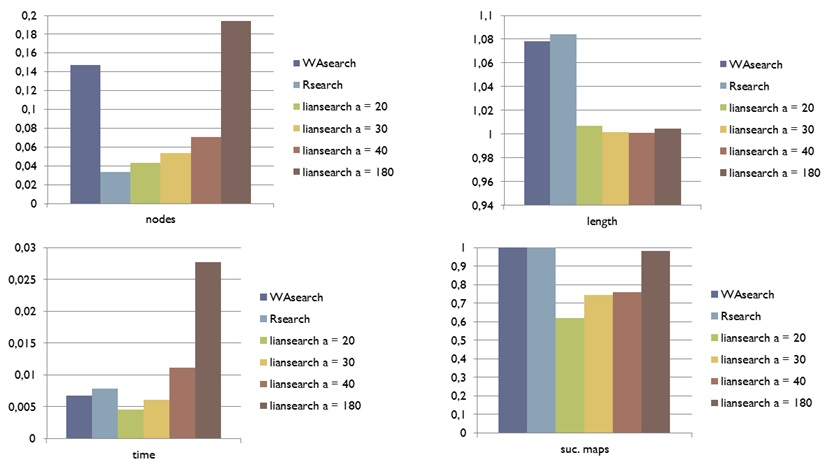
\includegraphics[width=\textwidth]{exp_plan_1.jpg}
		\end{figure}
	\end{frame}
	
	\section{Реактивный уровень}
	
	\begin{frame}
		\frametitle{Задача задачи робастного управления сложным техническим объектом}
		Вид управляемой нелинейной системы
		\begingroup
		\fontsize{9pt}{9pt}\selectfont
			\[\begin{matrix}
			\frac{dx}{dt}=\left( {{A}_{0}}+\varepsilon {{A}_{1}}(x,t) \right)x+\left( {{B}_{0}}+\varepsilon {{B}_{1}}(x,t) \right)u=({{A}_{cl}}+\,\,\varepsilon D(x,t,\varepsilon ))x=F(x,t,\varepsilon ),\\ x(0)={{x}_{0}}, \\ 
			x\in X\subset {{\text{R}}^{n}},u\in {{\text{R}}^{r}},t\in \left[ 0,\infty  \right),0<\varepsilon \le {{\varepsilon }_{0}} \\ 
			\end{matrix}\]
		\endgroup
		\par\bigskip
		I. Критерий оптимальности и общий вид формально оптимального управления для задачи синтеза робастного по параметру управления
		\begingroup
		\fontsize{9pt}{9pt}\selectfont
			\[\begin{matrix}
			I(u)=\frac{1}{2}\int_{0}^{\infty }{({{x}^{T}}Q(x,\varepsilon )x}+{{u}^{T}}R(x,\varepsilon )u)dt\to \min , \\ 
			u=-{{R}^{-1}}(x,\varepsilon ){{B}^{T}}(x,\varepsilon )K(x,\varepsilon )x,\quad  \\ 
			-K(x,\varepsilon )A(x,\varepsilon )-{{A}^{T}}(x,\varepsilon )K(x,\varepsilon )+K(x,\varepsilon )S(x,\varepsilon )K(x,\varepsilon )-Q(x,\varepsilon )=0, \\ 
			S(x,\varepsilon )=B(x,\varepsilon ){{R}^{-1}}(x,\varepsilon ){{B}^{T}}(x,\varepsilon ),R(x,\varepsilon ), \\ 
			Q={{Q}_{0}}+\varepsilon {{Q}_{1}}(x)+\ldots ,\quad K(x,\varepsilon )={{K}_{0}}+\varepsilon {{K}_{1}}(x),\quad R(x,\varepsilon )={{R}_{0}}+\varepsilon {{R}_{1}}(x). \\ 
			\end{matrix}\]
		\endgroup
	\end{frame}
	
	\begin{frame}
		\frametitle{Нелинейный закон управления}
		\begingroup
		\fontsize{9pt}{9pt}\selectfont
			\[\begin{matrix}
			-{{K}_{0}}{{A}_{0}}-{{A}_{0}}^{T}{{K}_{0}}+{{K}_{0}}{{S}_{0}}{{K}_{0}}-{{Q}_{0}}=0,\quad {{S}_{0}}={{B}_{0}}R_{0}^{-1}{{B}_{0}}^{T}.\\
			{{K}_{1}}(x)=\int\limits_{0}^{\infty }{\exp (({{A}_{0}}-{{S}_{0}}{{K}_{0}})_{{}}^{\text{T}}\sigma )}{{{\tilde{Q}}}_{1}}(x)\exp (({{A}_{0}}-{{S}_{0}}{{K}_{0}})\sigma )d\sigma ,\\ {{{\tilde{Q}}}_{1}}(x)>0\text{  }x\in X \\ 
			
			{{Q}_{2}}=-{{K}_{1}}\left( {{A}_{1}}-{{B}_{1}}{{R}_{0}}^{-1}B_{0}^{T}{{K}_{0}} \right)-{{\left( {{A}_{1}}-{{B}_{1}}{{R}_{0}}^{-1}B_{0}^{T}{{K}_{0}} \right)}^{T}}{{K}_{1}}+\\
			
			+\left( {{K}_{1}}{{B}_{0}}+{{K}_{0}}{{B}_{1}} \right){{R}_{0}}^{-1}{{\left( {{K}_{1}}{{B}_{0}}+{{K}_{0}}{{B}_{1}} \right)}^{T}}, \\ 
			
			{{Q}_{3}}={{K}_{1}}{{B}_{1}}{{R}_{0}}^{-1}{{\left( {{K}_{1}}{{B}_{0}}+{{K}_{0}}{{B}_{1}} \right)}^{T}}+\left( {{K}_{1}}{{B}_{0}}+{{K}_{0}}{{B}_{1}} \right){{R}_{0}}^{-1}{{B}_{1}}^{T}{{K}_{1}}, \\ 
			{{Q}_{4}}={{K}_{1}}{{B}_{1}}{{R}_{0}}^{-1}{{B}_{1}}^{T}{{K}_{1}}. \\ 
			\end{matrix}\]
		\endgroup
		II. Условие устойчивости замкнутой системы относительно одного класса нестационарных возмущений. 
		\begingroup
		\fontsize{9pt}{9pt}\selectfont
			\[\begin{matrix}
			\int_{{{t}_{0}}}^{{{t}_{0}}+l}{\varphi (\bar{x}(t,{{t}_{0}},{{x}_{0}},\varepsilon ),t,\varepsilon )}dt<\ \ -\delta {{\left\| {{x}_{0}} \right\|}^{d}}l,\quad d,\delta ,l=const, \\ 
			\varphi (\bar{x},t,\varepsilon )=\varepsilon {{x}_{0}}^{T}\exp (A_{cl}^{T}\cdot (t-{{t}_{0}})){{K}_{0}}D(\bar{x},t,\varepsilon )\exp ({{A}_{cl}}\cdot (t-{{t}_{0}})){{x}_{0}} \\ 
			\end{matrix}\]
		\endgroup
	\end{frame}
	
	\begin{frame}
		\frametitle{Примеры задач реактивного управления}

		1. Вывод продольных характеристик полета самолета вертикального взлета и посадки на заданный режим
		\begin{columns}
			\begin{column}{0.6\textwidth}
				\begingroup
				\fontsize{7pt}{7pt}\selectfont
					\[\begin{matrix}
					& {{{\dot{V}}}_{x}}=0.0174({{V}_{y}}{{\omega }_{z}}-g\vartheta )+{{C}_{x}}\rho S{{V}^{2}}+2\cdot {{10}^{-4}}{{P}_{}}+1.15\cdot {{10}^{-3}}{{P}_{}}, \\ 
					& {{{\dot{V}}}_{y}}=-0.0174{{V}_{x}}{{\omega }_{z}}+{{C}_{y}}\rho S{{V}^{2}}-g+1.14\cdot {{10}^{-3}}{{P}_{}}, \\ 
					& {{{\dot{\omega }}}_{z}}=-4.5\cdot {{10}^{-3}}V{{\omega }_{z}}+\varepsilon _{z}^{{{\delta }_{}}}{{\delta }_{}}, \\ 
					& \dot{\vartheta }={{\omega }_{z}}, \\ 
					\end{matrix}\]
				\endgroup				
			\end{column}
			\begin{column}{0.4\textwidth}
				\begin{figure}
					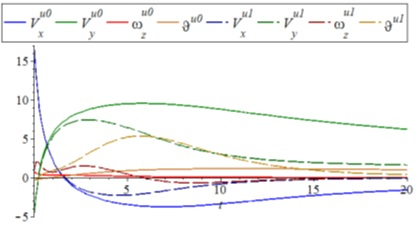
\includegraphics[width=0.7\textwidth]{control_res_1.jpg}
				\end{figure}
			\end{column}
		\end{columns}
		
		2. Управления абстрактной нелинейной системой второго порядка 
		
		\begin{columns}
			\begin{column}{0.5\textwidth}
				\begin{figure}
					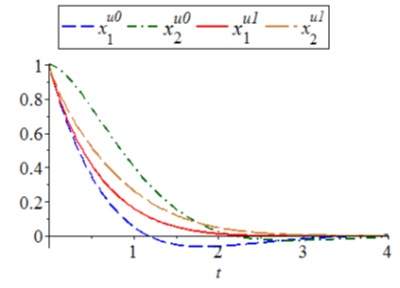
\includegraphics[width=0.7\textwidth]{control_res_2.jpg}
				\end{figure}
			\end{column}
			\begin{column}{0.5\textwidth}
				\begin{figure}
					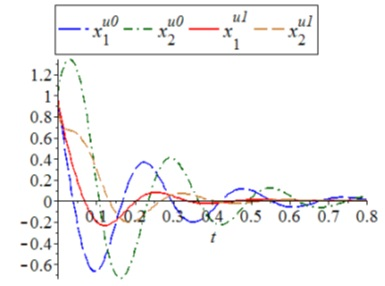
\includegraphics[width=0.7\textwidth]{control_res_3.jpg}
				\end{figure}
			\end{column}
		\end{columns}
	\end{frame}
\end{document}
	
